\chapter{Auswertung}
\label{ref:auswertung}
Nach Abschluss des Modelltrainings ist es essenziell, die Leistung der Modelle zu bewerten.
Das Ziel der Bewertung ist nicht nur zu analysieren, wie gut ein Modell auf die Trainingsdaten reagiert, sondern insbesondere, wie zuverlässig es auf unbekannte Daten verallgemeinert.
Gut auf unbekannte Daten zu reagieren wird auch die \enquote{Generalisierungsfähigkeit} genannt \cite{Goodfellow2016}.


%Train Test Split
Vor dem Training wurde für die Bewertung des Modells der Datensatz in Trainings- und Testdaten eingeteilt (Trainings- und Testsplitt).
Für die Leistungsbewertung wird der Testdatensatz verwendet, der dem Modell bisher nicht bekannt ist.
Nach Eingabe des Testdatensatzes in das Modell werden die Klassifizierungen mit den richtigen Entscheidungen verglichen.

Bei der Klassifizierung ist zu beachten, welche Klasse als positiv und welche als negativ definiert wird.  
Für die positive Klasse wird in dieser Arbeit die unterrepräsentierte Klasse verwendet, also diejenige, die seltener in den Daten vorkommt.  
Im Fall der Waitinglist betrifft dies die Ablehnung.  

Diese Entscheidung wurde getroffen, da eine ungleiche Klassenverteilung dazu führen kann, dass ein Modell bevorzugt die Mehrheitsklasse vorhersagt und die seltenere Klasse vernachlässigt.  
Durch die Wahl der unterrepräsentierten Klasse als positives Ereignis wird sichergestellt, dass die Bewertungsmetriken eine aussagekräftigere Interpretation ermöglichen, da sie verstärkt die Leistung des Modells in Bezug auf die seltenere Klasse widerspiegeln.

%\todo{IW: positv negativ bennenung (sehe ich anderns, muss ich belegen)}
%Man bezeichnet mit positiv normalerweise das wahrscheinlichere Ergebnis. Eine Ablehnung ist also wahrscheinlicher als eine Annahme.


%\todo{IW: Fehlern von erklärung der Waitinglist in der Grundlage}
%Sie haben bisher nirgendwo erklärt, welche Fälle Sie bei Waitingslists unterscheiden wollen und welche Klassen Sie vorhersagen wollen.
%Das gehört eindeutig zum fachlichen Wissen, das für diese Arbeit hier relevant ist und muss daher ganz vorne beschrieben werden.

%Überleitung
%Damit kann man nun Statistiken erstellen, wie viel ein Modell in bestimmten Bereichen leistet. 

\pagebreak
\section{Bewertungsmetriken}

%\todo{IW: Ist so ok?}
%Das ist jetzt wieder Grundlagenwissen. Da Sie das aber erst hier wirklich brauchen (nämlich in der Auswertung), finde ich ok, dass Sie das hier auch erst erklären.

Verschiedenste Bewertungsmetriken helfen dabei, die Leistung zu bewerten.

%Es wurde schon der Loss vorgestellt. Dieser ist aber keine Bewertungsmetrik, sowie nicht automatisch mit anderen Loss-Werten vergleichbar, wenn beispielsweise andere Loss-Funktionen verwendet wurden. Daher werden noch weitere Metriken benötigt. 

%\todo{IW: Loss ist keine Bewertungsmetrik}
%Die Verlustfunktion, die Sie bisher vorgestellt haben, ist nur von Relevanz, um beim Backpropagation-Algorithmus die Gewichte anzupassen.
%Sie erwecken den Eindruck, dass die Verlustfunktion eine Alternative zu den Bewertungsmetriken ist. Das ist aber gar nicht so.
%Hier geht es nämlich gar nicht um die Implementierung einer Neuronalen-Netz-Technik, sondern allgemein um eine statistische Bewertung der Vorhersagequalität. Das müssen Sie auch bei der Random-Forest-Methode machen, und Sie machen das nachher ja auch.

Um viele Metriken auszurechnen, muss erstmals eine Konfusionsmatrix aufgestellt werden \cite{Swaminathan2024}. 
Dabei wird jedes Ereignis sowohl danach kategorisiert, ob sie tatsächlich positiv oder negativ ist, als auch danach, ob sie als positiv oder negativ vorhergesagt wurde \cite{Swaminathan2024}.
\begin{table}[H]
    \centering
    \konfusionstabular[]{Wahr positiv ($TP$)}{Falsch negativ ($FN$)}{Falsch positiv ($FP$)}{Wahr negativ ($TN$)}
    \caption{Konfusionsmatrix}
    \label{tab:confusion_matrix}
\end{table}

Hierbei ist zu beachten, dass unsere Modelle eine Wahrscheinlichkeit $p$ zwischen $0$ und $1$ ausgeben. Wobei $1$ für $100\%$ Ablehnung-Einschätzung und $0$ für $100\%$ Annahme-Einschätzung steht. Dadurch wird die Ablehnung mit einem Schwellwert von $0,5$ definiert. Eine Ablehnung ist also immer mit $p \geq 0\text{,}5$ definiert. 
Das bedeutet, dass das Modell eine Ablehnung vorhersagt, wenn es für eine Waitinglist-Entscheidung einen Wert größer als $0\text{,}5$ ausgibt.

Um die richtigen Metriken zu wählen, wurde systematisch vorgegangen.
Zur Bewertung wurden verschiedene Metriken betrachtet, wobei für diejenigen, bei denen es möglich war, eine spezifische Fragestellung formuliert wurde, um ihre Aussagekraft zu beschreiben:

\begin{enumerate}
    \item \textbf{Genauigkeit (Accuracy)}: Diese Metrik ist zunächst die offensichtlichste. Hierbei wird die Frage beantwortet: \textbf{Wie viel Prozent der Entscheidungen wurden richtig klassifiziert?}. Wenn die Entscheidungen nicht ausgeglichen sind, ist die Metrik nicht aussagekräftig. Beispiel: Nehmen wir an, die Verteilung von Annahme zu Ablehnung bei der Waitinglist ist $20\%$ Ablehnung und $80\%$ Annahme. Wenn das Modell nur Annahmen vorhersagt, würde es trotzdem eine $80\%$ Genauigkeit erzielen, obwohl keine einzige Ablehnung korrekt klassifiziert wurde. Mathematisch ist die Genauigkeit wie folgt definiert \cite{Swaminathan2024}: \[\text{Genauigkeit} = \frac{(TP + TN)}{(TP + FN + FP + TN)}\]
    Es werden alle richtigen Vorhersagen durch alle Entscheidungen geteilt. Aufgrund der Limitationen wird die Genauigkeit oft mit weiteren Metriken kombiniert \cite{Goodfellow2016}.
    
    \item \textbf{Präzision (Precision)}: Diese Metrik gibt an, wie viele der als positiv vorhergesagten Ereignisse tatsächlich korrekt klassifiziert wurden. Im Fall der Waitinglist beantwortet die Präzision die Frage: \textbf{Wie viele der als Ablehnung vorhergesagten Entscheidungen werden tatsächlich abgelehnt?} 
    Mathematisch drückt sich das wie folgt aus \cite{Swaminathan2024}:  \[\text{Präzision} = \frac{TP}{TP + FP}\]
    Die Metrik ist im Fall der Waitinglist interessant, da die Entscheidung der Ablehnung möglichst richtig sein muss. 
    Falsch positive Ergebnisse, in dem Fall die Ablehnungen, bedeuten hierbei potenziellen finanziellen Verlust. 
    Als Beispiel können wir ein Zwischenergebnis des Trainings anhand der folgenden Konfusionsmatrix betrachten:
    \begin{table}[H]
        \centering
        \konfusionstabular[]{$78188$ ($TP$)}{$31611$ ($FN$)}{$147142$ ($FP$)}{$460788$ ($TN$)}
        \caption{Beispiel: Konfusionsmatrix mit niedriger Präzision}
        \label{tab:confusion_matrix_1}
    \end{table}
    Hier ergibt sich eine Präzision von: \[ \text{Präzision} = \frac{78188}{78188 + 147142} = 34\text{,}7\% \]
    Obwohl die Genauigkeit mit $75\%$ relativ hoch erscheint, zeigt die niedrige Präzision, dass von dem Modell als Ablehnung eingestufte Vorhersagen nur selten richtig sind und damit potenziell finanzielle Verluste verursachen. 
    Allerdings gibt diese Metrik keinerlei Auskunft darüber, wie viele Ablehnungen tatsächlich erkannt wurden. 
    Wenn ein Modell nahezu keine positiven Ereignisse vorhersagt, ist diese Metrik nicht aussagekräftig. 
    
    \item \textbf{Sensitivität (Recall)}: Während die Präzision beschreibt, wie viele der vorhergesagten positiven Ereignisse tatsächlich richtig sind, beantwortet die Sensitivität, wie viele aller tatsächlichen positiven Ereignisse erkannt wurden. 
    Im Fall der Waitinglist wird die folgende Frage beantwortet: \textbf{Wie gut ist das Modell darin, Ablehnungen zu klassifizieren?}. Mathematisch ist die Sensitivität wie folgt definiert \cite{Swaminathan2024}: \[\text{Sensitivität}=\frac{TP}{TP + FN}\] 
    Die Sensitivität ist besonders wichtig in Anwendungsfällen, in denen es entscheidend ist, möglichst viele positive Ereignisse zu erkennen. Ein Beispiel dafür ist die medizinische Diagnostik, wo es besser ist, fälschlicherweise gesunde Patienten als krank zu klassifizieren, anstatt kranke Patienten zu übersehen \cite{Hastie2009}.
    Im Fall der Waitinglist ist die Sensitivität zwar relevant, da unerkannte Ablehnungen zu logistischen Problemen führen können, jedoch wird sie hier als weniger kritisch als die Präzision betrachtet. Da Schiffe häufig überbucht werden, ist eine hohe Präzision wichtiger, um finanzielle Verluste zu vermeiden.
    
    \item \textbf{F1-Wert}: Der F1-Wert \textbf{kombiniert Präzision und Sensitivität} in einer einzigen Kennzahl, die als harmonisches Mittel der beiden Werte berechnet wird. Er ist besonders dann sinnvoll, wenn sowohl Präzision als auch Sensitivität von Bedeutung sind, ohne eine der beiden Metriken zu bevorzugen. Mathematisch ist der F1-Wert definiert als \cite{Swaminathan2024}: \[\text{F1-Wert}=\frac{2 \cdot TP}{2 \cdot TP + FP + FN}\]
    Der F1-Wert ist insbesondere bei unausgeglichenen Datensätzen eine nützliche Bewertungsmetrik. Da bei der Waitinglist sowohl Präzision als auch Sensitivität hohe Relevanz haben, wird der F1-Wert genutzt, um die Gesamtleistung des Modells zu bewerten. 

    \item \textbf{\gls{roc} - Kurve} / \textbf{\gls{auc}}: Eine besonders wichtige Metrik für binäre Klassifikationsprobleme. Bei allen bis jetzt gezeigten Metriken wurde die Vorhersage der Modelle nur als entweder angenommen oder abgelehnt betrachtet. Dies wurde durch den Schwellwert $0\text{,}5$ entschieden.  
    Die \gls{roc}-Kurve hingegen betrachtet die Modellvorhersagen als Wahrscheinlichkeiten und zeigt die Leistung des Modells über verschiedene Schwellenwerte hinweg. Sie stellt die \gls{tpr} gegen die \gls{fpr} dar \cite{Swaminathan2024}:

    \begin{figure}[H]
        \centering
        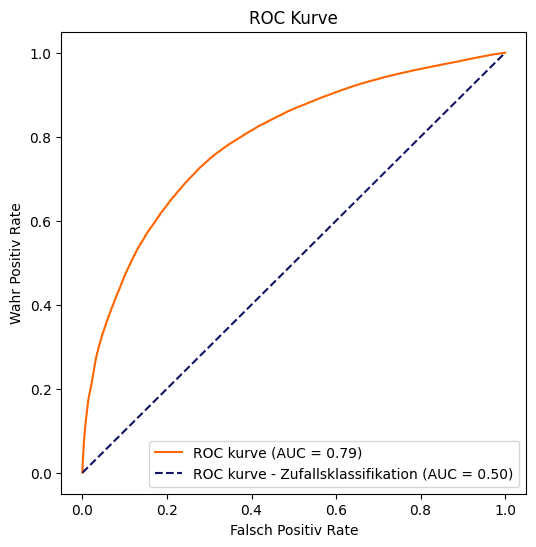
\includegraphics[width=0.5\linewidth]{Thesis//bilder/ROC-Bad.png}
        \caption{ROC-Kurve}
        \label{fig:roc_bad}
    \end{figure}

    Durch das Variieren des Schwellenwerts kann die Sensitivität gegen die \gls{fpr} aufgetragen werden, wodurch die ROC-Kurve entsteht. Ein ideal funktionierendes Modell würde eine Kurve aufweisen, die möglichst weit oben links in der Grafik verläuft, da dies bedeutet, dass es eine hohe Sensitivität bei einer gleichzeitig niedrigen \gls{fpr} erreicht.

    Die Fläche unter der \gls{roc}-Kurve ergibt dabei den \gls{auc}-Wert. 
    Dieser gibt an, \textbf{wie gut das Modell zwischen den Klassen trennt}.

    Bei der \cref{fig:roc_bad} ist die \textcolor{hlblue}{\textit{blau-gestrichelte Linie}}, die \gls{roc}-Kurve, die Zufallsentscheidungen repräsentiert. Die \textcolor{hlorange}{\textit{orange Linie}} ist ein Modell, welches noch Verbesserungspotenzial hat. 
    Dabei entscheidet das \textcolor{hlorange}{Modell} deutlich besser als ein \textcolor{hlblue}{Zufallsgenerator}.
    Das kann mittels der \gls{auc}-Werte, sowie des Kurvenverlaufes abgelesen werden.
    
    Da die Ablehnung einer Buchung finanzielle Auswirkungen haben kann, ist es wichtig, ein Gleichgewicht zwischen \gls{tpr} und \gls{fpr} zu finden. Ein hoher AUC-Wert bedeutet, dass das Modell gut zwischen angenommenen und abgelehnten Buchungen unterscheiden kann.
\end{enumerate}

\clearpage
\section{Modellmetriken}
\label{sec:model_results}
Die vorgestellten Metriken können verwendet werden, um die Leistung der \gls{ml}-Modelle zu bewerten.
Die Ergebnisse können auf dem beigefügten Datenträger, in den entsprechenden Notebooks, verifiziert werden.  
\paragraph{Neuronales Netz}
Das finale neuronale Netz erreichte folgende Werte:
\begin{itemize}[noitemsep]
    \item \textbf{Genauigkeit (Accuracy)}: $86\text{,}85\%$
    \item \textbf{Präzision (Precision)}: $84\text{,}78\%$
    \item \textbf{Sensitivität (Recall)}: $76\text{,}08\%$
    \item \textbf{F1-Wert}: $80\text{,}20\%$
    \item \textbf{\gls{auc}}: $91\text{,}59\%$
\end{itemize}



Die \textbf{Genauigkeit von 86,85\%} zeigt, dass das Modell insgesamt eine hohe Vorhersagequalität besitzt. 
Allerdings ist die Genauigkeit alleine nicht immer aussagekräftig, insbesondere beim unausgeglichenen Datensatz.

Die \textbf{Präzision von 84,78\%} bedeutet, dass $84\text{,}78\%$ der vorhergesagten positiven Ereignisse (Ablehnungen) tatsächlich korrekt sind. Dies ist besonders wichtig, da falsch-positive Vorhersagen zu nicht gewollten Ablehnungen führen können, die in der Praxis finanzielle Verluste verursachen könnten.

Die \textbf{Sensitivität (Recall) von 76,08\%} gibt an, dass das Modell $76\text{,}08\%$ aller tatsächlichen positiven Ereignisse erkannt hat. Dies bedeutet, dass etwa $23\text{,}92\%$ der abgelehnten Buchungen nicht korrekt vorhergesagt wurden. Eine höhere Sensitivität wäre wünschenswert, um die Anzahl falsch angenommener Buchungen zu minimieren.


Der \textbf{F1-Wert von 80,20\%} stellt den Kompromiss zwischen Präzision und Sensitivität dar. Dies zeigt, dass das Modell ein gutes Gleichgewicht zwischen der korrekten Identifikation von Ablehnungen und der Vermeidung von Fehlklassifikationen findet.
Hier ist aber noch Verbesserungspotenzial vorhanden.

Die \textbf{\gls{auc} von 91,59\%} verdeutlicht, dass das Modell eine sehr hohe Trennfähigkeit zwischen den Klassen besitzt. Ein Wert über $90\%$ zeigt, dass das Modell gut darin ist, zwischen angenommenen und abgelehnten Buchungen zu unterscheiden, unabhängig von der gewählten Schwelle.


\paragraph{Random Forest}
Für den Random Forest wurden folgende Werte erreicht:
\begin{itemize}[noitemsep]
    \item \textbf{Genauigkeit (Accuracy)}: $93\text{,}53\%$
    \item \textbf{Präzision (Precision)}: $92\text{,}37\%$
    \item \textbf{Sensitivität (Recall)}: $86\text{,}37\%$
    \item \textbf{F1-Wert}: $89\text{,}27\%$
    \item \textbf{\gls{auc}}: $97\text{,}62\%$
\end{itemize}

Die \textbf{Genauigkeit von 93,53\%} ist im Vergleich zum neuronalen Netz um $6\text{,}68\%$ höher.

Die \textbf{Präzision von 92,37\%} ist sogar um $7\text{,}59\%$ höher. Die vorhergesagten positiven Ereignisse (Ablehnungen) sind tatsächlich häufiger korrekt.

Die \textbf{Sensitivität (Recall) von 86,37\%} hat dabei den größten Anstieg von $10\text{,}29\%$, es werden dabei also auch $10\text{,}29\%$ mehr Ablehnungen erkannt.

Dies äußert sich auch im höheren \textbf{F1-Wert von 89,27\%}.
Verdeutlicht wird dies durch den \textbf{\gls{auc} von 97,62\%}, der auch um $5\text{,}07\%$ gestiegen ist. Das Modell kann also noch deutlich besser als das neuronale Netz zwischen angenommenen und abgelehnten Buchungen unterscheiden. 

\paragraph{Logistische Regression}
Bei der logistischen Regression wurden folgende Werte erreicht:
\begin{itemize}[noitemsep]
    \item \textbf{Genauigkeit (Accuracy)}: $79\text{,}73\%$
    \item \textbf{Präzision (Precision)}: $73\text{,}24\%$
    \item \textbf{Sensitivität (Recall)}: $55\text{,}13\%$
    \item \textbf{F1-Wert}: $62\text{,}90\%$
    \item \textbf{\gls{auc}}: $84\text{,}25\%$
\end{itemize}

Dies sind die niedrigsten Werte.
Die \textbf{Genauigkeit von 79,73\%} ist im Vergleich zum neuronalen Netz um $7\text{,}12\%$ niedriger.
Weniger Waitinglist-Entscheidungen werden richtig vorhergesagt.

Die \textbf{Präzision von 73,24\%} ist dementsprechend auch um $11\text{,}54\%$ gesunken.
Die logistische Regression ist also deutlich schlechter darin, die Ablehnungen richtig vorherzusagen.

Die \textbf{Sensitivität (Recall) von 55,13\%} ist um $20\text{,}95\%$ gesunken. Das ist der schlechteste Sensitivitätswert, der erreicht wurde. 
Es wird also fast nur die Hälfte aller Ablehnungen erkannt.

Zusammengefasst im \textbf{F1-Wert von 62,90\%} zeigen sich auch der gesunkene Präzisions- und Sensitivitätswert.
Der \textbf{\gls{auc} von 84,25\%} spiegelt wider, dass die logistische Regression im Vergleich mit dem Random Forest und dem neuronalen Netz deutlich schlechter zwischen den angenommenen und abgelehnten Buchungen trennt. 


%\todo{IW: Versuchsreihen, verifizirung?}
%Wo sind denn die Versuchsreihen dazu, um das verifizieren zu können?
%Analog bei Random Forest.

\paragraph{Interpretation}
Bei der Auswertung zeigt sich, dass die logistische Regression am schlechtesten abschneidet. Da nur knapp mehr als die Hälfte der Ablehnungsvorhersagen richtig erkannt werden, ist diese Methode keine geeignete Wahl.
Das neuronale Netz erkennt diese deutlich besser und wäre grundsätzlich für eine Empfehlung an die Mitarbeiter geeignet, jedoch erzielt das weniger komplexe Random Forest-Modell bei geringem Implementationsaufwand deutlich bessere Ergebnisse.
%\todo{IW: Warum ist NN eine valide wahl}
%Das kann ich diesem gar nicht entnehmen:
%Warum einfach, wenn es auch kompliziert geht, oder was?
%Welche Vorteile hat denn ein neuronales Netz?

Dies ist nicht nur an einem Wert festzustellen, sondern alle Werte sind höher als bei dem neuronalen Netz und der logistischen Regression. 
Das Random Forest-Modell übertrifft die beiden Methoden in sämtlichen Metriken und sagt die Waitinglist-Entscheidungen somit präziser voraus.

%Dieses Ergebnis könnte an dem unausgewogenen Datensatz entstanden sein, da das Random Forest-Modell weniger Daten benötigt, um bessere Ergebnisse zu erzielen.
%Vielleicht Overfitting -> Muss noch der Loss des Trainings dem Test set übergegengestellt werden



%Neurale netzte performen schelchter wenn der datensatz unausgewogen ist wahrscheinlich
%Ist das Ergebnis überraschend?
%Warum ist der unterschied so groß. Warum ist Wert x bei RF größer als bei NN


%\todo{Interpretation der ergebnisse weiter schreiben}